\documentclass[12pt,a4paper]{report}

\usepackage{alltt, fancyvrb, url}
\usepackage{graphicx}
\usepackage[utf8]{inputenc}
\usepackage{float}
\usepackage{xcolor}
\usepackage{hyperref}
\usepackage{listings}

\definecolor{codegreen}{rgb}{0,0.6,0}
\definecolor{codegray}{rgb}{0.5,0.5,0.5}
\definecolor{codepurple}{rgb}{0.58,0,0.82}
\definecolor{backcolour}{rgb}{0.95,0.95,0.92}

\lstdefinestyle{mystyle}{
    backgroundcolor=\color{backcolour},   
    commentstyle=\color{codegreen},
    keywordstyle=\color{magenta},
    numberstyle=\tiny\color{codegray},
    stringstyle=\color{codepurple},
    basicstyle=\ttfamily\footnotesize,
    breakatwhitespace=false,         
    breaklines=true,                 
    captionpos=b,                    
    keepspaces=true,                 
    numbers=left,                    
    numbersep=5pt,                  
    showspaces=false,                
    showstringspaces=false,
    showtabs=false,                  
    tabsize=2
}
\lstset{style=mystyle}

\usepackage{enumitem}
\usepackage{amsmath}
\usepackage{geometry}
\geometry{margin=1in}

\usepackage{newlfont}
\usepackage{gensymb}

\usepackage[italian]{babel}
\usepackage[italian]{cleveref}

\graphicspath{ {./src/img} }

\textwidth=450pt\oddsidemargin=0pt
\begin{document}

\begin{titlepage}
\begin{center}
{{\Large{\textsc{Alma Mater Studiorum $\cdot$ Università di Bologna}}}} \rule[0.1cm]{15.8cm}{0.1mm}
\rule[0.5cm]{15.8cm}{0.6mm}
{\small{\bf CORSO DI LAUREA IN INGEGNERIA E SCIENZE INFORMATICHE \\ A.A. 2024/25 }}
\end{center}
\vspace{15mm}
\begin{center}
{\LARGE{\bf Analisi del traffico ICMP e TCP}}\\
\vspace{2mm}
{\LARGE{\bf con Scapy e Wireshark}}
\end{center}
\begin{center}
{\LARGE Relazione per il corso di Programmazione di Reti}
\end{center}

\vspace{8mm}
\begin{center}

\includegraphics[width=0.65\textwidth]{Copertina}
\end{center}
\vspace{15mm}

{\large{\bf \noindent
Presentato da:\\}
Bartocetti Enrico, 0001115097}
\end{titlepage}

\tableofcontents

\chapter{Introduzione}

\subsubsection{Obiettivo}
Creare e inviare pacchetti ICMP e TCP con Scapy, catturarli con Wireshark e analizzare i risultati.

\subsubsection{Requisiti minimi}
\begin{itemize}
	\item Inviare pacchetti ICMP Echo (ping) e TCP SYN verso un host
	\item Catturare i pacchetti in Wireshark e salvarli in .pcap
	\item Analizzare: IP di origine/destinazione, porte, checksum, TTL
\end{itemize}

\subsubsection{Estensioni}
\begin{itemize}
	\item Inviare un pacchetto TCP con flag personalizzati
	\item Visualizzare e spiegare le differenze tra ICMP e TCP
	\item Generare un semplice report HTML o PDF con gli screen e analisi
\end{itemize}

\subsubsection{Output atteso}

\begin{itemize}
	\item Script Python con Scapy (\texttt{/src/script.py})
	\item File .pcap della cattura (presenti nella cartella \texttt{/wireshark})
	\item Relazione con screenshot e commenti tecnici
\end{itemize}

\chapter{Pacchetti ICMP Echo}

\section{Generazione dei pacchetti con Scapy}

Si vuole inviare un pacchetto \texttt{ICMP Echo Request} (ping) a un host. Per l'invio ho utilizzato il metodo \texttt{.sr()} della libreria scapy, specificando il tipo \texttt{ICMP}. Riporto nel Listing \ref{code:icmp} la funzione che ho scritto per poter generare il pacchetto del ping, che richiede come parametro l'indirizzo IP oppure l'hostname del destinatario. La funzione stampa anche il risultato dell'operazione.

\begin{lstlisting}[language=Python, caption={Funzione python per la generazione di un pacchetto \texttt{ICMP Echo Request}}, label={code:icmp}]
import scapy.all as scapy

def send_ping(destination):
    print("----- INVIO PING A", destination, " -----")
    res = scapy.sr(scapy.IP(dst=destination)/scapy.ICMP(), timeout=4) 
    print("--- RISULTATI: ---")
    for r in res:
        r.show()
    print()
\end{lstlisting}

\section{Analisi del traffico con Wireshark}
Ho mandato il ping a \texttt{google.com}, che è stato risolto nell'indirizzo IP \texttt{216.58.204.238}.\\
Per la cattura del traffico di rete ho utilizzato wireshark con il filtro \texttt{host 216.58.204.238} per catturare solo i pacchetti da / per l'host indicato. Nel file \texttt{wireshark/icmp{\textunderscore}echo.pcap} è presente il risultato della cattura. \\
Riporto in seguito il dettaglio della richiesta e della risposta.

\subsection{ICMP Echo Request}
\label{subsection:ICMPEchoRequest}

\begin{figure}[H]
	\centering
	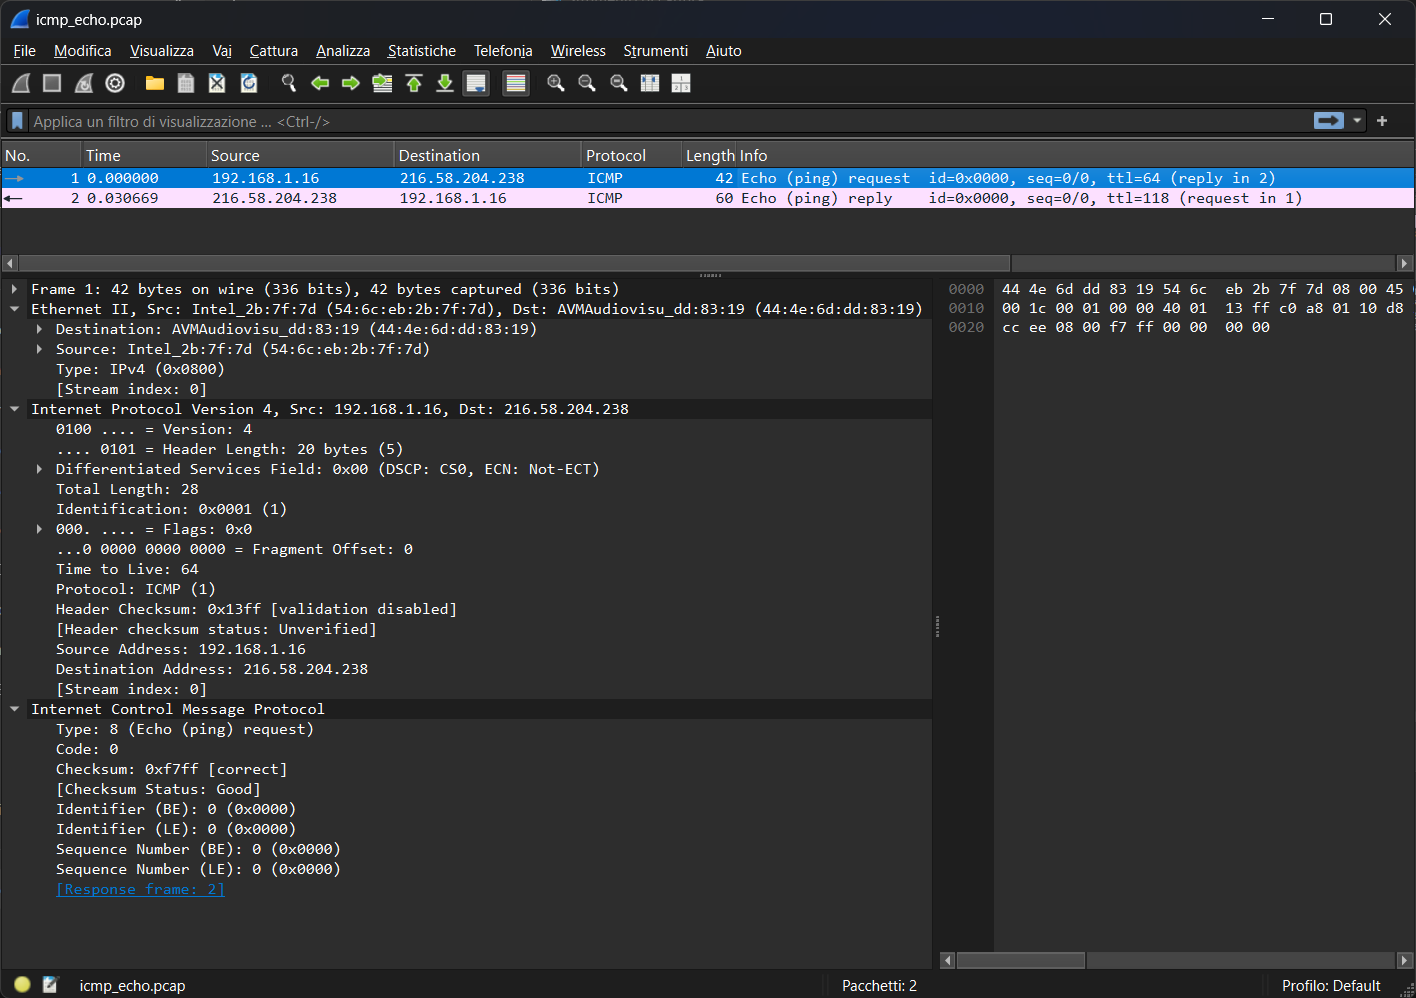
\includegraphics[width=1\textwidth]{icmp_echo_request}
 	\caption{Dettaglio Wireshark dell'Echo Request}
\end{figure}
Il pacchetto parte dal mio PC connesso alla rete di casa, infatti nella PCI del livello IP troviamo il campo \texttt{Source Address: 192.168.1.16}, ovvero l'IP privato del mio PC nella mia rete. Nel campo \texttt{Destination Address: 216.58.204.238} troviamo l'IP del destinatario della richiesta, ovvero l'host verso cui ho inviato il pacchetto ping. Il campo Time To Live è settato al livello massimo (64) visto che il pacchetto è stato catturato non appena generato.\\
Nella parte dati del pacchetto IP viene trasportato il pacchetto ICMP: possiamo confermarlo leggendo il campo \texttt{Protocol: ICMP} nell'header del pacchetto IP. All'interno della parte riservata al protocollo ICMP viene specificato che il pacchetto è di tipo \texttt{Echo Request}.\\
Notiamo che non sono presenti riferimenti a nessuna porta: questo perché IP e ICMP sono protocolli dell'Internet Layer della suite TCP/IP , quindi non c'è la necessità di comunicare tramite una porta con un livello superiore (ovvero con un protocollo di trasporto).\\
Risulta infine evidente che sia il pacchetto IP sia quello ICMP sono dotati di un proprio checksum, che nel caso dell'IP non viene verificato mentre nell'ICMP è corretto. 

\subsection{ICMP Echo Reply}
\begin{figure}[H]
	\centering
	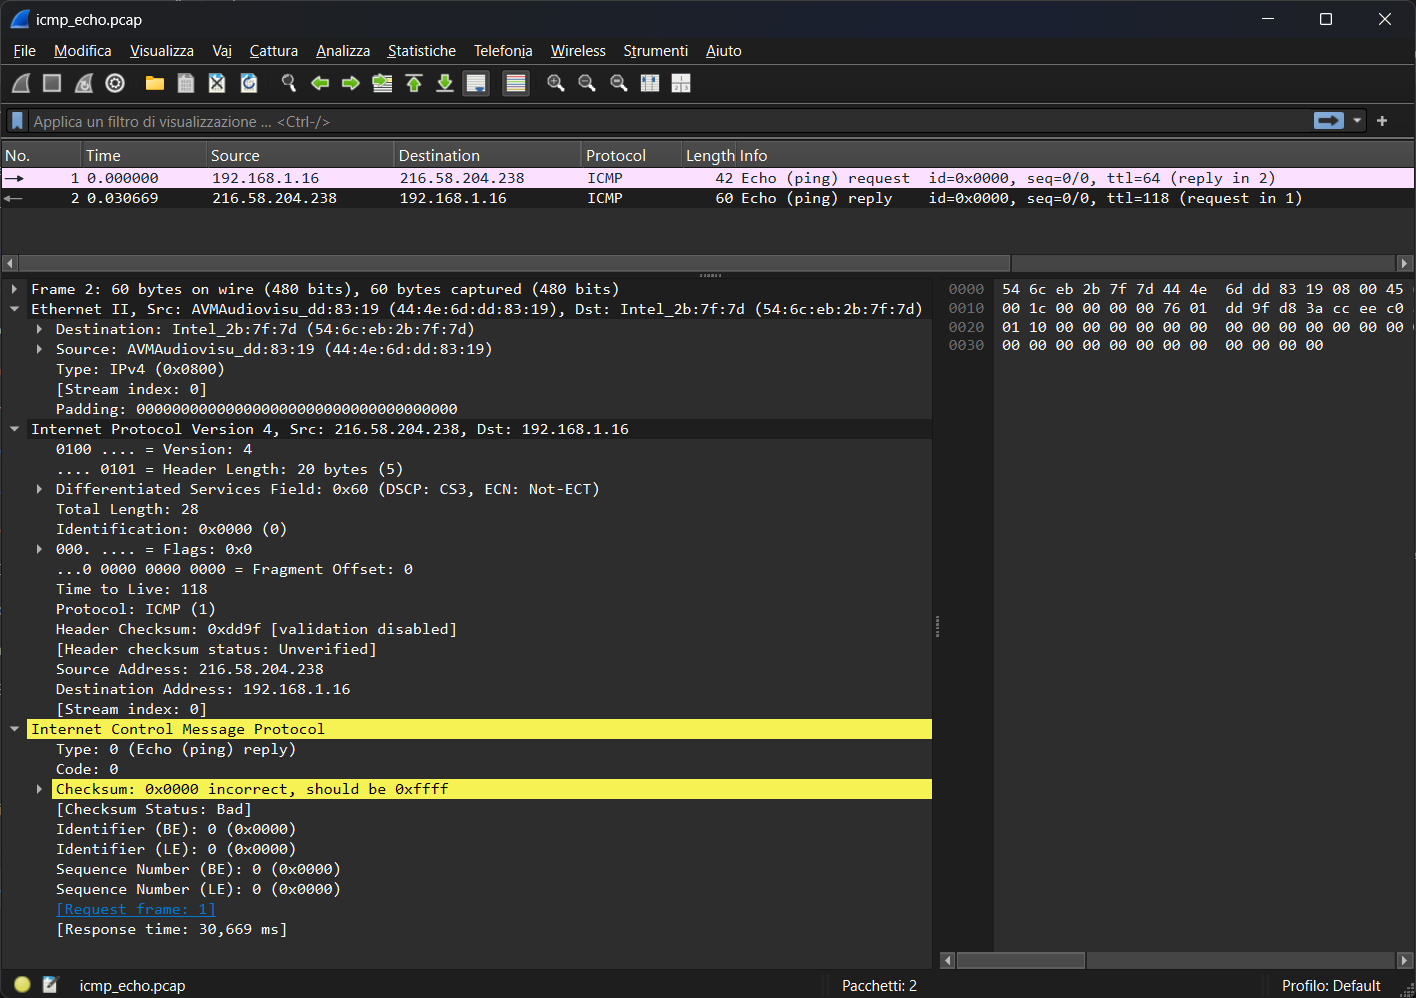
\includegraphics[width=1\textwidth]{icmp_echo_reply}
 	\caption{Dettaglio Wireshark dell'Echo Reply}
\end{figure}
Questa cattura presenta varie differenze rispetto a quella precedente. 
Quella più ovvia è l'inversione degli indirizzi IP nei campi \texttt{Destination Address: 192.168.1.16} e  \texttt{Source Address: 216.58.204.238}, visto che si tratta del pacchetto di risposta (quindi generato dal destinatario del ping).\\
Poiché si tratta della risposta al ping iniziale, IP ci dice che il protocollo utilizzato è sempre \texttt{Protocol: ICMP}, mentre nella parte riservata al protocollo ICMP viene specificato che si tratta di una \texttt{Echo Reply}.\\
In questo caso il campo {TTL} è settato a 118: possiamo presupporre che alla generazione del pacchetto sia stato 128 (la potenza del 2 più vicina a 118), ma è stato decrementato di un'unita per ogni router che il pacchetto ha attraversato.
Utilizzando il comando \texttt{tracert 216.58.204.238} ho poi verificato che per raggiungere il destinatario dal mio host sono necessari 10 salti. \\
Come prima il checksum dell'header IP è presente ma non verificato. Nel caso di ICMP invece, si ha che il checksum calcolato è diverso da quello riportato nel pacchetto. Ho provato a ripetere varie volte il ping, ottenendo sempre lo stesso risultato: potrebbe quindi essere che l'host destinatario sceglie di non calcolare il checksum lasciandolo a 0. Il contenuto informativo del pacchetto sembra comunque essere corretto nei campi che sono di nostri interesse.

\chapter{Segmenti TCP SYN}

\section{Generazione dei pacchetti con Scapy}
Si vuole inviare un segmento \texttt{TCP} con il flag \texttt{SYN} a un host: ciò corrisponde alla richiesta di instaurazione di una connessione. \\
Come nel capitolo precedente, ho utilizzato il metodo \texttt{.sr()} della libreria scapy, specificando il tipo \texttt{TCP}, con il flag \texttt{S} attivo (ovvero SYN). Riporto nel Listing \ref{code:tcp_syn} la funzione che ho scritto per poter generare il pacchetto contenente il segmento TCP, che richiede come parametro l'indirizzo IP (o l'hostname) e la porta del destinatario. La funzione stampa anche il risultato dell'operazione.

\begin{lstlisting}[language=Python, caption={Funzione python per la generazione di un segmento \texttt{TCP} con flag \texttt{SYN} attivo}, label={code:tcp_syn}]
import scapy.all as scapy

def send_tcp_syn(destination, port):
    print("----- INVIO SYN A", destination, ", PORTA", port, "-----")
    res = scapy.sr(scapy.IP(dst=destination)/scapy.TCP(dport=port,flags="S"), timeout=4)
    print("--- RISULTATI: ---")
    for r in res:
        r.show()
    print()
\end{lstlisting}

\section{Analisi del traffico con Wireshark}
\begin{figure}[H]
	\centering
	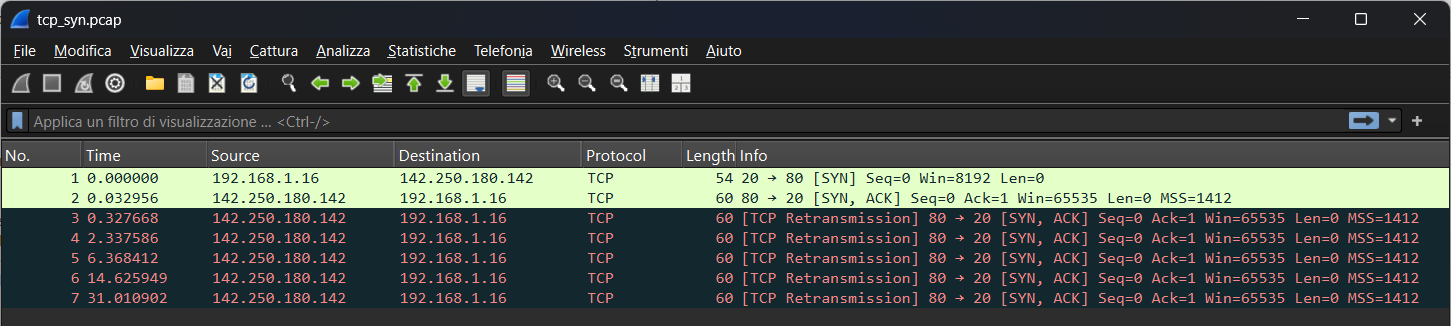
\includegraphics[width=1\textwidth]{tcp_syn_capture}
 	\caption{Pacchetti catturati da Wireshark}
	\label{tcp_syn_capture}
\end{figure}
Visto che un TCP SYN dà il via al three way handshake, per considerare la connessione instaurata è necessario che l'host da cui parte la richiesta confermi con un ACK finale. Nel nostro caso ciò non avviene, infatti notiamo che il server ritrasmette periodicamente il suo \texttt{SYN ACK} (vedi Figura \ref{tcp_syn_capture}), credendo che quelli precedenti siano stati perduti durante la trasmissione. \\
Il file della cattura contenente i pacchetti sniffati su cui sono stati effettuati gli screenshot, è il file \texttt{/wireshark/tcp{\textunderscore}syn.pcap} .

\subsection{Richiesta TCP con SYN attivo}
\begin{figure}[H]
	\centering
	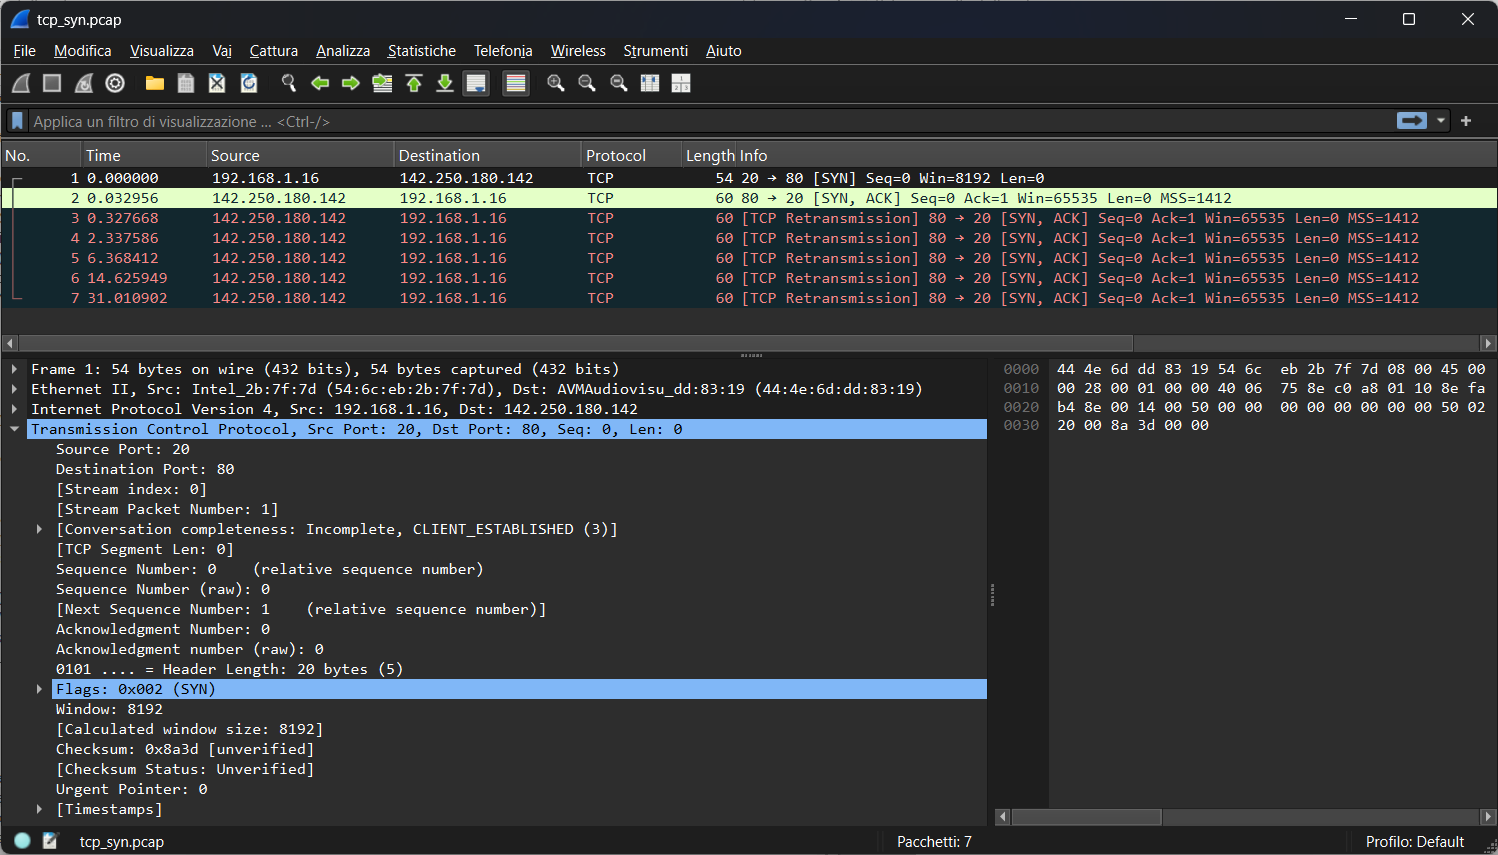
\includegraphics[width=1\textwidth]{tcp_syn_request}
 	\caption{Dettaglio del pacchetto trasmesso, con flag SYN attivo}
	\label{tcp_syn_request}
\end{figure}
\begin{figure}[H]
	\centering
	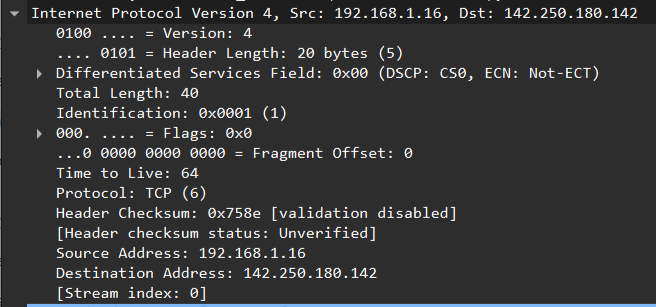
\includegraphics[width=0.5\textwidth]{tcp_syn_request_ip_layer}
 	\caption{Dettaglio dell'header IP}
	\label{tcp_syn_request_ip_layer}
\end{figure}
Controlliamo innanzitutto l'header del protocollo IP (vedi Figura \ref{tcp_syn_request_ip_layer}).
Come nell'analisi precedente (vedi sezione \ref{subsection:ICMPEchoRequest}) il \texttt{Source Address} e il \texttt{Time To Live} sono rimasti invariati; è rimasta disabilitata anche la validazione dell'header.
Il \texttt{Destination Address} contiene un indirizzo IP diverso rispetto al precedente, nonostante io abbia mandato il pacchetto sempre a \texttt{google.com}: questo è successo perché il server DNS ha ritenuto opportuno risolvere lo stesso nome di dominio con un altro indirizzo, probabilmente per poter distribuire meglio il carico sui vari server.
Grazie al campo \texttt{Protocol: TCP} notiamo che nel payload del pacchetto viene trasportato un segmento del protocollo TCP, che andremo ad analizzare (il cui contenuto viene riportato in Figura \ref{tcp_syn_request}.) \\
Per essere sicuro di comunicare con un server TCP ho scelto come \texttt{Destination Port: 80}: questo perché 80 è il numero di porta well-known attribuito ai server HTTP, e l'HTTP è un protocollo applicativo che utilizza il protocollo TCP a livello di trasporto.
Il campo \texttt{Source Port: 20} ci dice che scapy ha scelto di utilizzare la porta 20 TCP del mio PC per la comunicazione: probabilmente viene scelta di default quando non si specifica una porta sorgente.
Questo non dovrebbe però accadere visto che la porta 20 corrisponde alla well-known port per il trasferimento dei dati del protocollo applicativo FTP; avrebbe invece dovuto utilizzare una porta libera (nel range 49152 - 65535) assegnata dal sistema operativo, visto che i client quando instaurano una connessione non hanno bisogno di utilizzare una porta nota. Anche in questo caso il checksum riportato non viene verificato.

\subsection{Risposta TCP con SYN ACK attivi}
\begin{figure}[H]
	\centering
	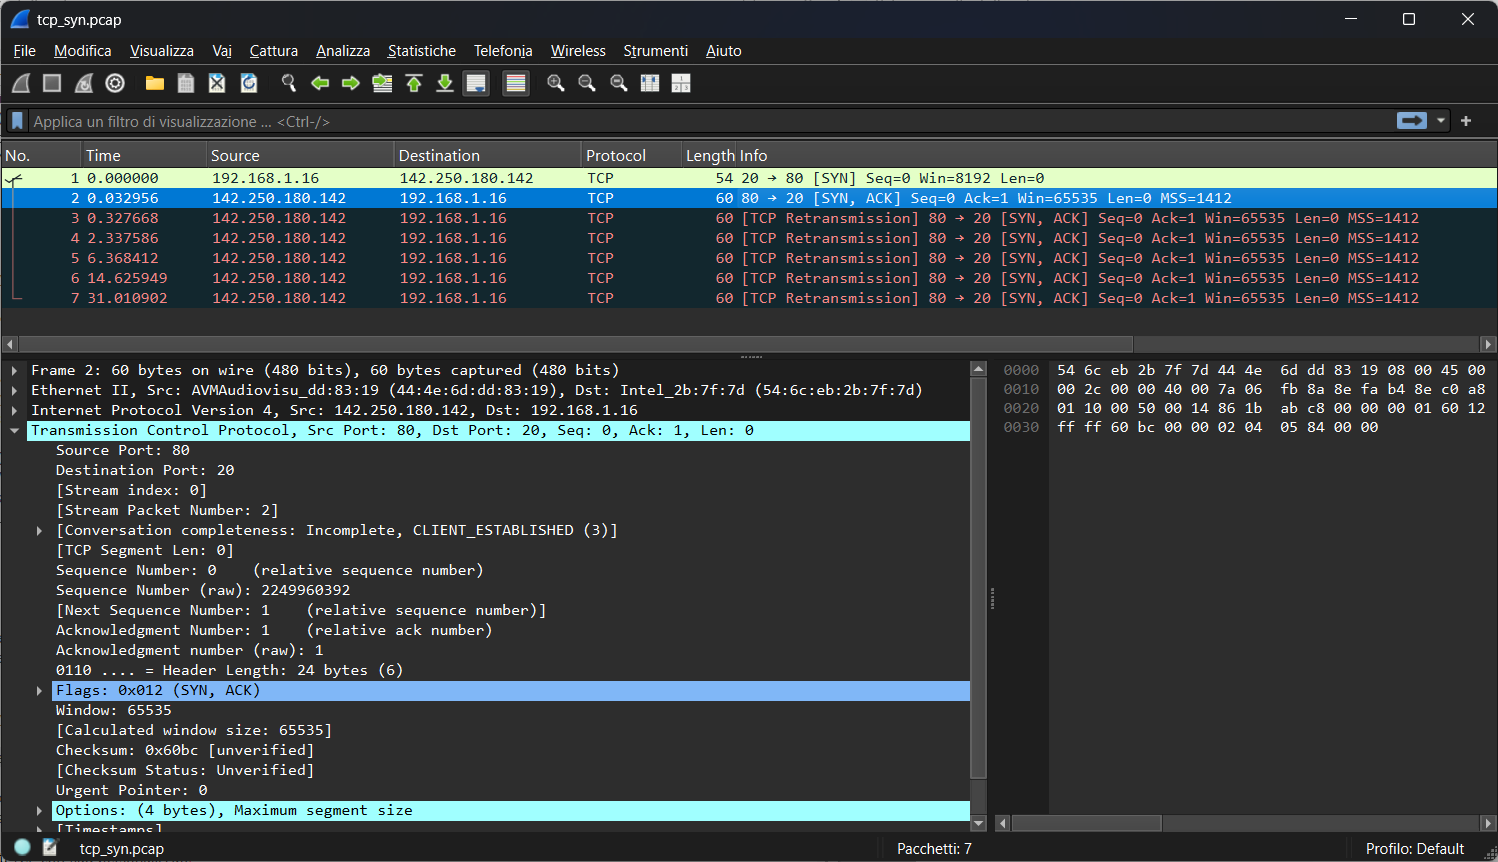
\includegraphics[width=1\textwidth]{tcp_syn_ack_reply}
 	\caption{Dettaglio del pacchetto ricevuto con flag SYN e ACK attivi}
	\label{tcp_syn_ack_reply}
\end{figure}
\begin{figure}[H]
	\centering
	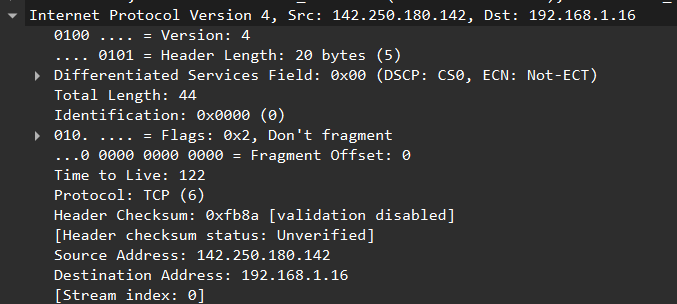
\includegraphics[width=0.5\textwidth]{tcp_syn_ack_reply_ip_layer}
 	\caption{Dettaglio dell'header IP}
	\label{tcp_syn_ack_reply_ip_layer}
\end{figure}
Visto che si tratta del pacchetto di risposta alla mia richiesta di connessione (Figura \ref{tcp_syn_ack_reply_ip_layer}), gli indirizzi IP riportati sono gli stessi ma scambiati tra mittente e destinatario. Notiamo sempre che il TTL è stato decrementato di qualche unità, che il protocollo della PDU trasportata nei dati del pacchetto IP è il protocollo TCP e che il checksum non è stato verificato. \\
Passando all'analisi del protocollo TCP (Figura \ref{tcp_syn_ack_reply}), trattandosi della risposta, anche qua le porte sorgente e destinatario sono scambiate.
Poiché questo segmento è il secondo step del three way handshake, vediamo che sono attivi i flag \texttt{SYN} e \texttt{ACK}: il server ci sta confermando tramite l'ACK di aver ricevuto la nostra richiesta di connessione, e contemporaneamente chiede al mio host di aprire la connessione inviando il SYN.
L'ACK number è impostato a 1 per confermare al mio PC di aver ricevuto correttamente tutti i segmenti con numero di sequenza fino allo 0, quindi il prossimo che si aspetta è il segmento con numero di sequenza a 1. 
Il numero di sequenza del server invece parte da 2249960392, ovvero un numero generato in maniera casuale per evitare di avere segmenti dispersi per la rete con lo stesso sequence number che potrebbero essere ricevuti quando non hanno più nessun senso, dando origine a vari errori.

\subsection{Ritrasmissioni TCP con SYN ACK attivi}
\begin{figure}[H]
	\centering
	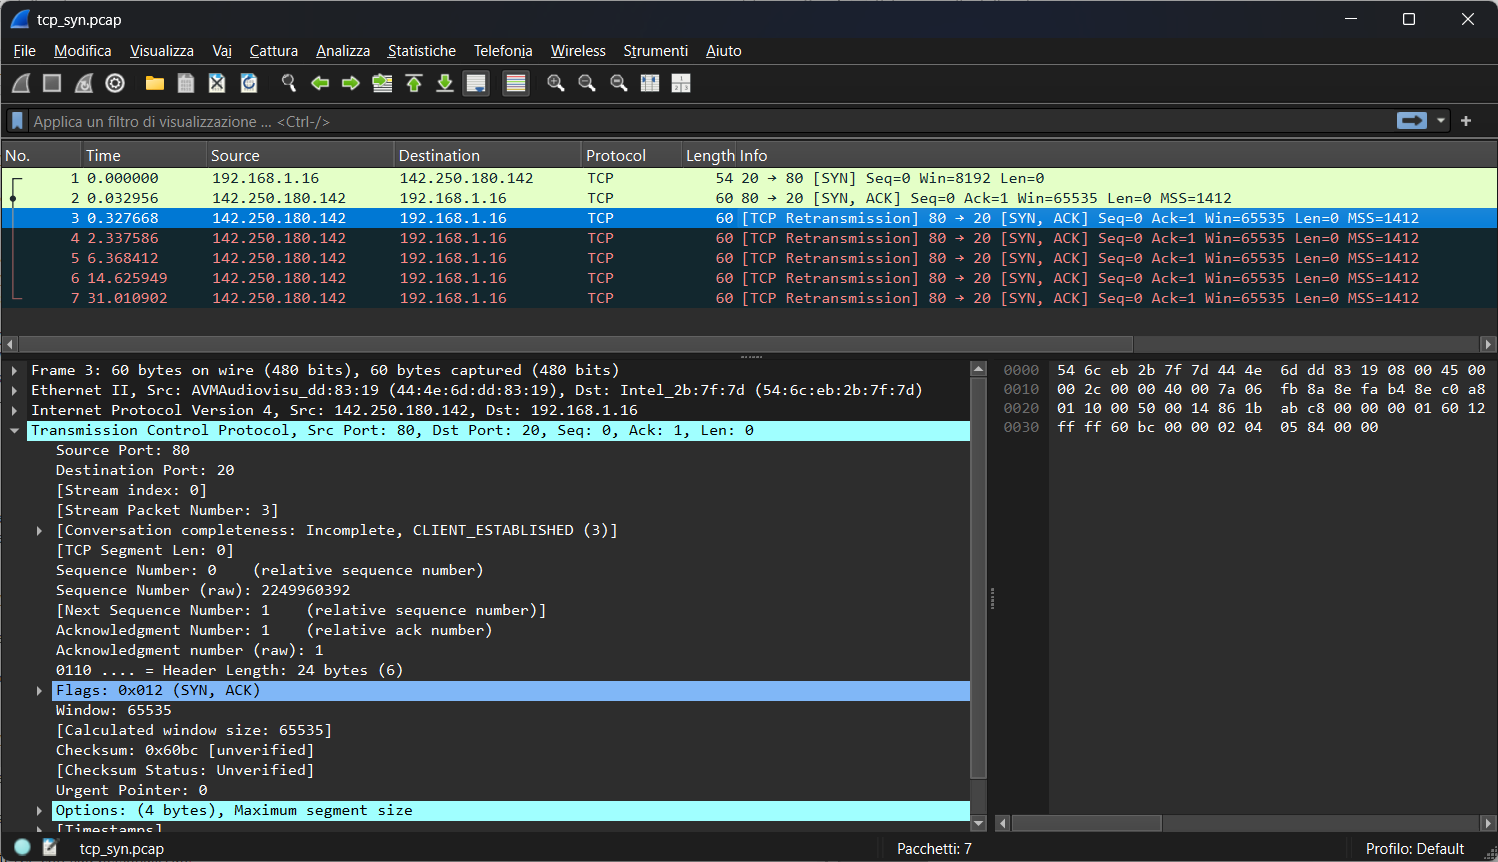
\includegraphics[width=1\textwidth]{tcp_syn_ack_retransmission}
 	\caption{Dettaglio del pacchetto ricevuto in seguito alla ritrasmissione, con flag SYN e ACK attivi}
	\label{tcp_syn_ack_retransmission}
\end{figure}
Il codice python contenuto nel Listing \ref{code:tcp_syn} invia un TCP SYN e riceve l'eventuale risposta, senza però effettuare nient'altro.
Il three way handshake si considera concluso (e quindi la connessione è stabilita) solo dopo la conferma finale data dall'host richiedente all'host destinatario con un segmento con flag ACK attivo, segmento che il mio host non invia al server.
Per questo motivo il server crede che il suo SYN ACK non sia mai arrivato a destinazione, causando così la ritrasmissione dello stesso (notiamo infatti che tutto il contenuto del segmento è uguale a quello precedente, vedi Figura \ref{tcp_syn_ack_reply}) allo scadere del tempo di timeout.

\chapter{Segmenti TCP con flag personalizzati}

\section{Generazione dei pacchetti con Scapy}
La generazione di segmenti TCP attivando flag personalizzati è resa molto semplice dalla libreria scapy: è sufficiente creare una stringa conentente un carattere per ogni flag scelto, come riportato nel Listing \ref{code:tcp_flags}.
Ad esempio per attivare i flag FIN e ACK bisogna settare \texttt{flags="FA"}. \\
Nella funzione che ho scritto, lascio scegiere all'utente quali flag vuole abilitare.

\begin{lstlisting}[language=Python, caption={Funzione python per la generazione di un segmento \texttt{TCP} con flag attivabili a scelta}, label={code:tcp_flags}]
import scapy.all as scapy

def send_tcp_flags(destination, port):
    print("----- FLAG DISPONIBILI: -----")
    print("F - FIN")
    print("S - SYN")
    print("R - RST")
    print("P - PSH")
    print("A - ACK")
    print("U - URG")
    print("E - ECE")
    print("C - CWR")
    print("\nDigitare i caratteri dei flag da attivare (ad esempio \"SR\" per i flag SYN e RST)\n>", end=" ")
    flgs = input().upper()
    print("----- INVIO FLAG", flgs, "A", destination, ", PORTA", port, "-----")
    res = scapy.sr(scapy.IP(dst=destination)/scapy.TCP(dport=port,flags=flgs), timeout=4)
    print("--- RISULTATI: ---")
    for r in res:
        r.show()
    print()
\end{lstlisting}

\section{Analisi del traffico con Wireshark}

\subsection{Tutti i flag attivi}
\begin{figure}[H]
	\centering
	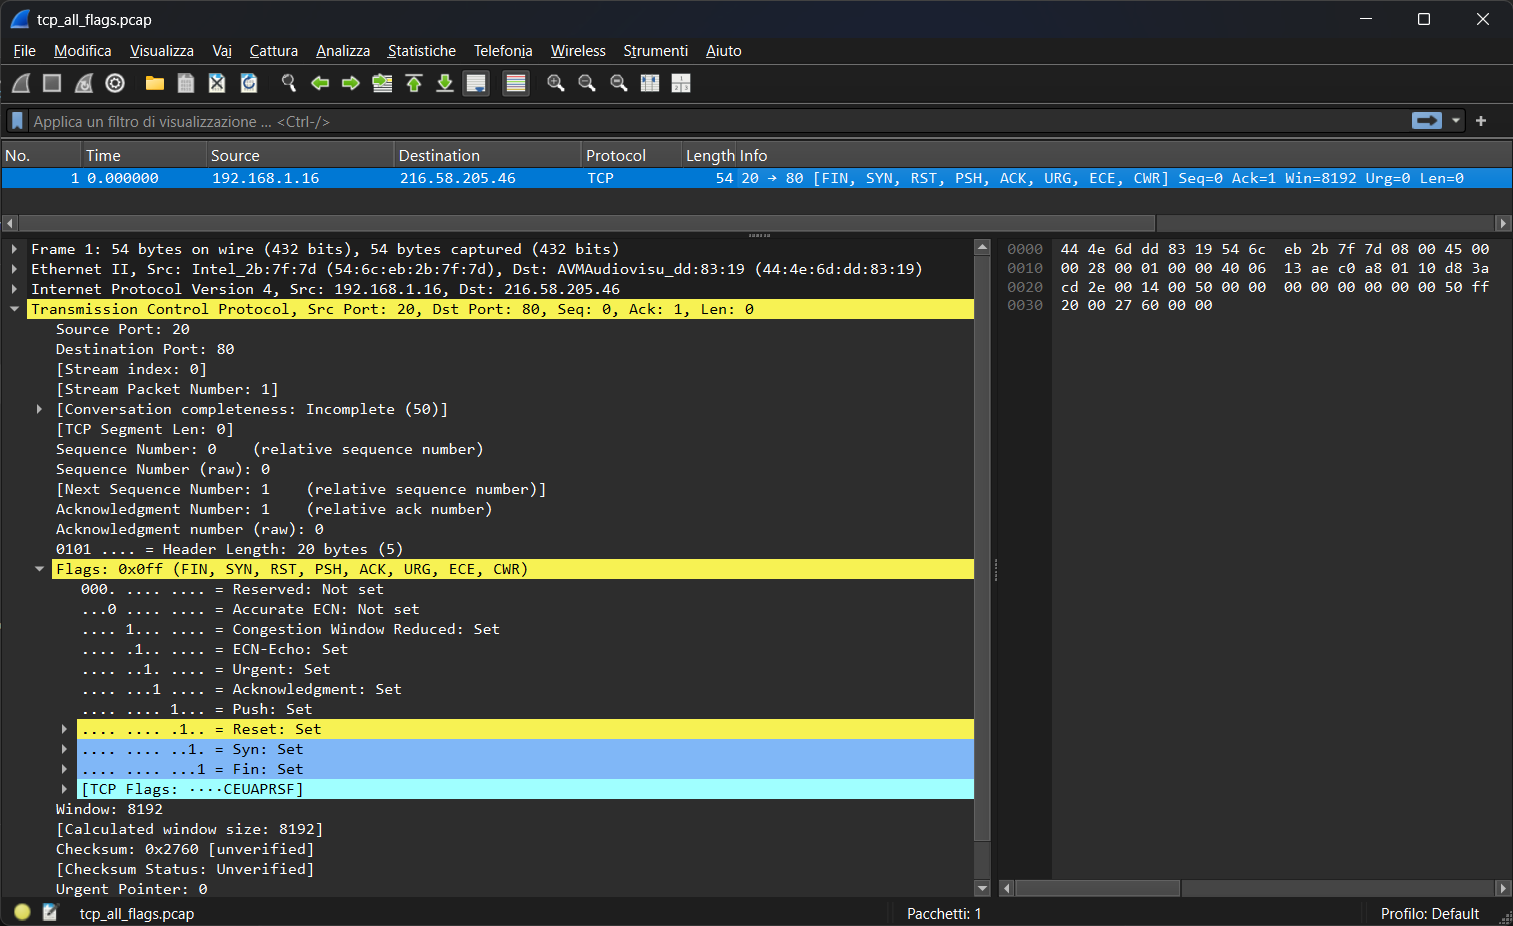
\includegraphics[width=1\textwidth]{tcp_all_flags}
 	\caption{Dettaglio del pacchetto inviato con tutti i flag attivi}
	\label{tcp_all_flags}
\end{figure}
Tramite la funzione sopra descritta, ho inviato un segmento TCP al server HTTP \texttt{google.com:80} abilitando tutti i flag possibili.
Questa operazione non ha ovviamente alcun senso, infatti dalla cattura si vede che non ho ricevuto nessuna risposta dal server. 
Il pacchetto è salvato nel file \texttt{/wireshark/tcp{\textunderscore}all{\textunderscore}flags.pcap} .

\subsection{Three-way handshake}
\begin{figure}[H]
	\centering
	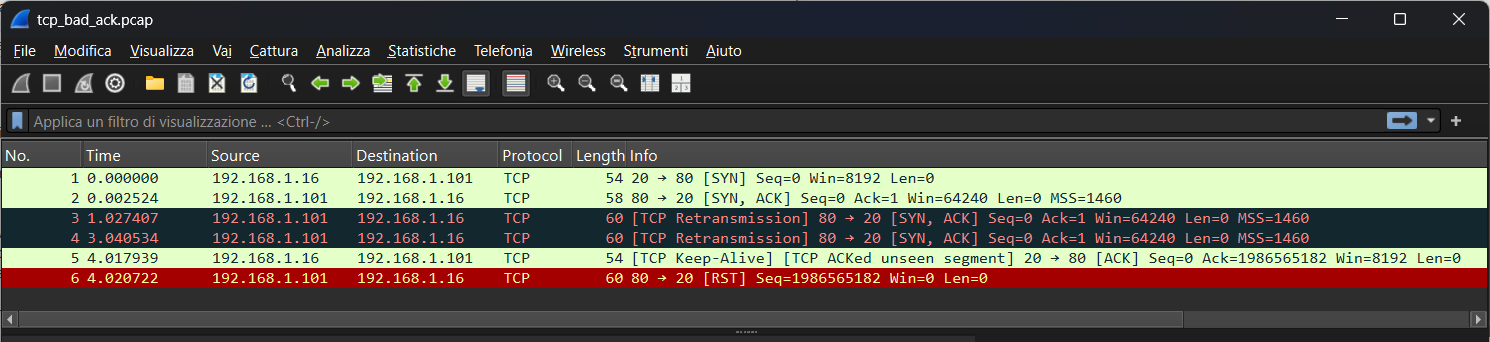
\includegraphics[width=1\textwidth]{tcp_bad_ack_packets}
 	\caption{Sequenza dei pacchetti inviati nel tentativo di simulare un three-way handshake}
	\label{tcp_bad_ack}
\end{figure}
In questa prova ho cercato di simulare un three-way handshake con un mio server HTTP: riporto punto per punto la spiegazione di ogni pacchetto riferendomi al numero progressivo riportato dalla cattura di wireshark.
\begin{enumerate}
	\item Ho generato un segmento con il flag SYN attivo, per far partire il three-way handshake
	\item Il server conferma la sua disponibilità ad aprire la connessione inviando un segmento con SYN e ACK attivi
	\item Poiché stavo generando i pacchetti a mano con lo script, ho impiegato un po' di tempo per generare l'ACK di risposta, causando la scadenza del tempo di timeout del server (ovvero credeva che il suo pacchetto SYN ACK si fosse perso per la rete)
	\item Come il punto 3
	\item Questo segmento contiene l'ACK che ho generato, che avrebbe dovuto terminare il three-way handshake confermando l'apertura della connessione
	\item Visto che il pacchetto generato al punto 5 contiene il flag di ACK ma ha sequence number e ack number errati, il server risponde con un segmento contenente il flag RST per resettare la connessione poiché si sono verificati questi errori nella numerazione dei segmenti
\end{enumerate}
Il risultato della cattura di whireshark è salvato nel file \texttt{/wireshark/tcp{\textunderscore}bad{\textunderscore}ack.pcap} .

\chapter{Commenti finali}
\section{Differenze tra ICMP e TCP}
ICMP e TCP sono due protocolli completamente differenti: il primo appartiene al \textbf{livello 3} del modello ISO/OSI (livello rete del TCP/IP), il secondo al \textbf{livello 4} ISO/OSI (livello di trasporto del TCP/IP).
Mentre ICMP è utilizzato per ottenere informazioni diagnostiche dalla rete (abbiamo visto che possiamo eseguire il ping verso un host per verificarne la raggiungibilità), TCP è utilizzato per garantire affidabilità (controllo di flusso, rilevazione di errore, controllo della congestione, ecc...) instaurando una connessione basata su un livello per sua natura inaffidabile, ovvero il livello rete.
Abbiamo infine notato che nel segmento TCP abbiamo indicate le porte del mittente e del destinatario, mentre nei pacchetti ICMP no: questo è dovuto al fatto che TCP è un protocollo di livello superiore rispetto ad IP, quindi le porte sono le SAP (Service Access Point) che mettono in comunicazione il livello 3 con il livello 4.

\end{document}